\section{\thesection.~Examples}

\begin{frame}{}
    \fullcite{Harasim2020}
\end{frame}

\begin{frame}{Research questions}
    \begin{enumerate}
        \item How can the concept of a mode be operationalized? 
        \item How can we find modes automatically? 
        \item Can we do it without knowing how many modes there are and what they look like?
        \item How do modes change historically?
    \end{enumerate}
\end{frame}

\begin{frame}{Corpus}
    \begin{figure}
        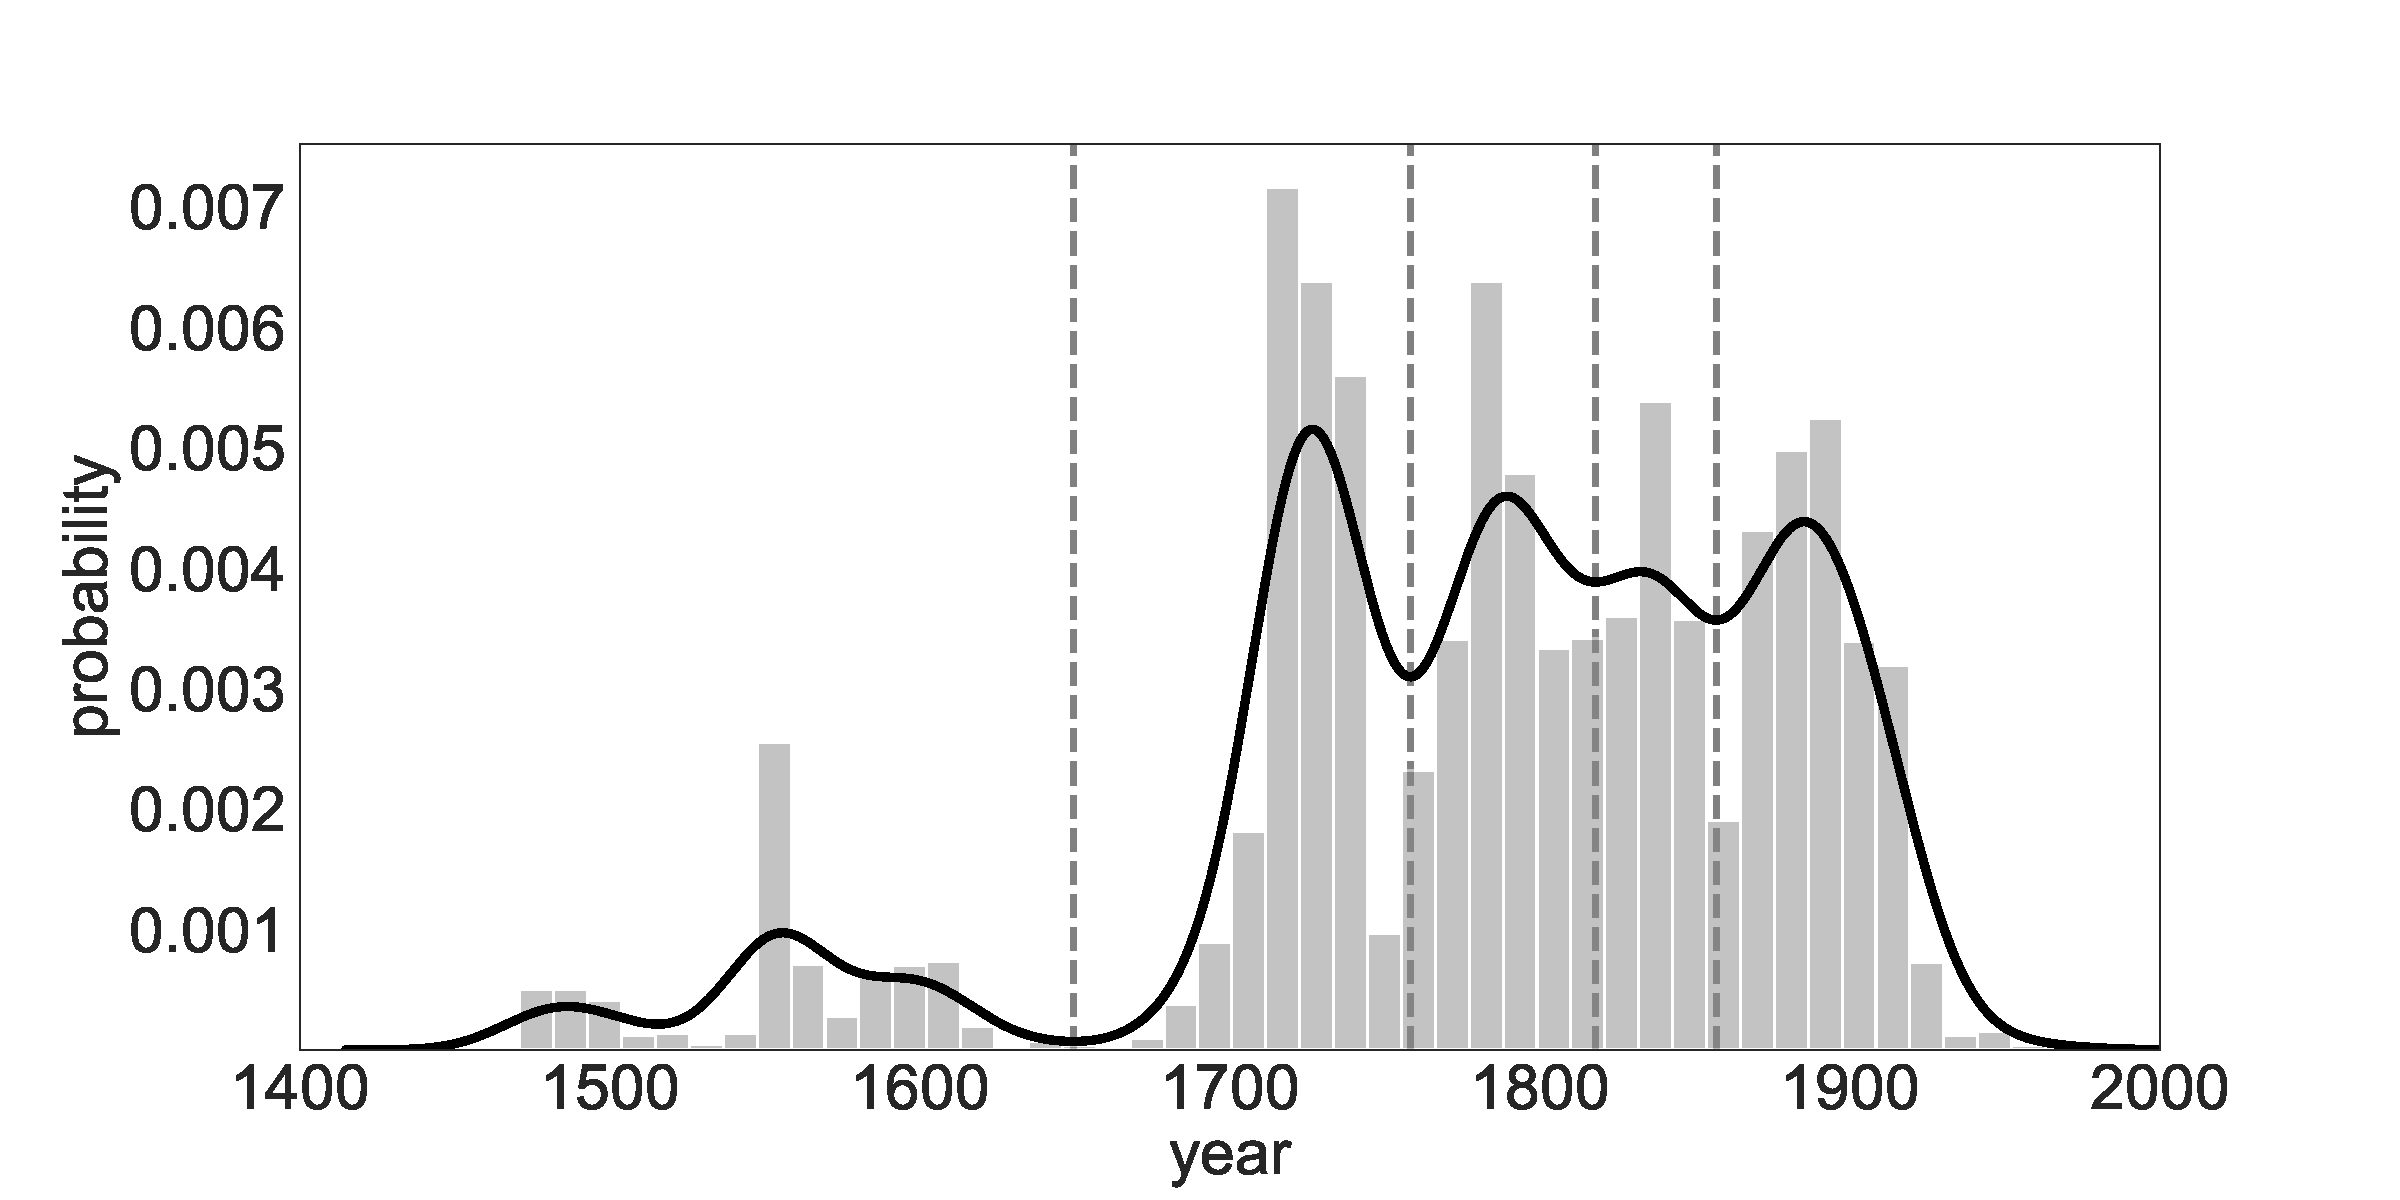
\includegraphics[width=\linewidth,height=.8\textheight,keepaspectratio]{img/Figure1.pdf}
        \caption{Historical distribution of pieces in the corpus.}
        \label{fig:piece_dist}
    \end{figure}
\end{frame}

\begin{frame}{The model and its assumptions}
    \begin{enumerate}
        \item pieces can be represented by pitch-class counts
        \item enharmonic equivalence
        \item transpositional invariance
    \end{enumerate}

    \pause
    
    All of these assumptions are highly questionable, especially on a large historical scale!
    
    \pause
    
    $\Longrightarrow$ explitic modeling
\end{frame}

\begin{frame}{Automatically finding modes}
    \begin{figure}
        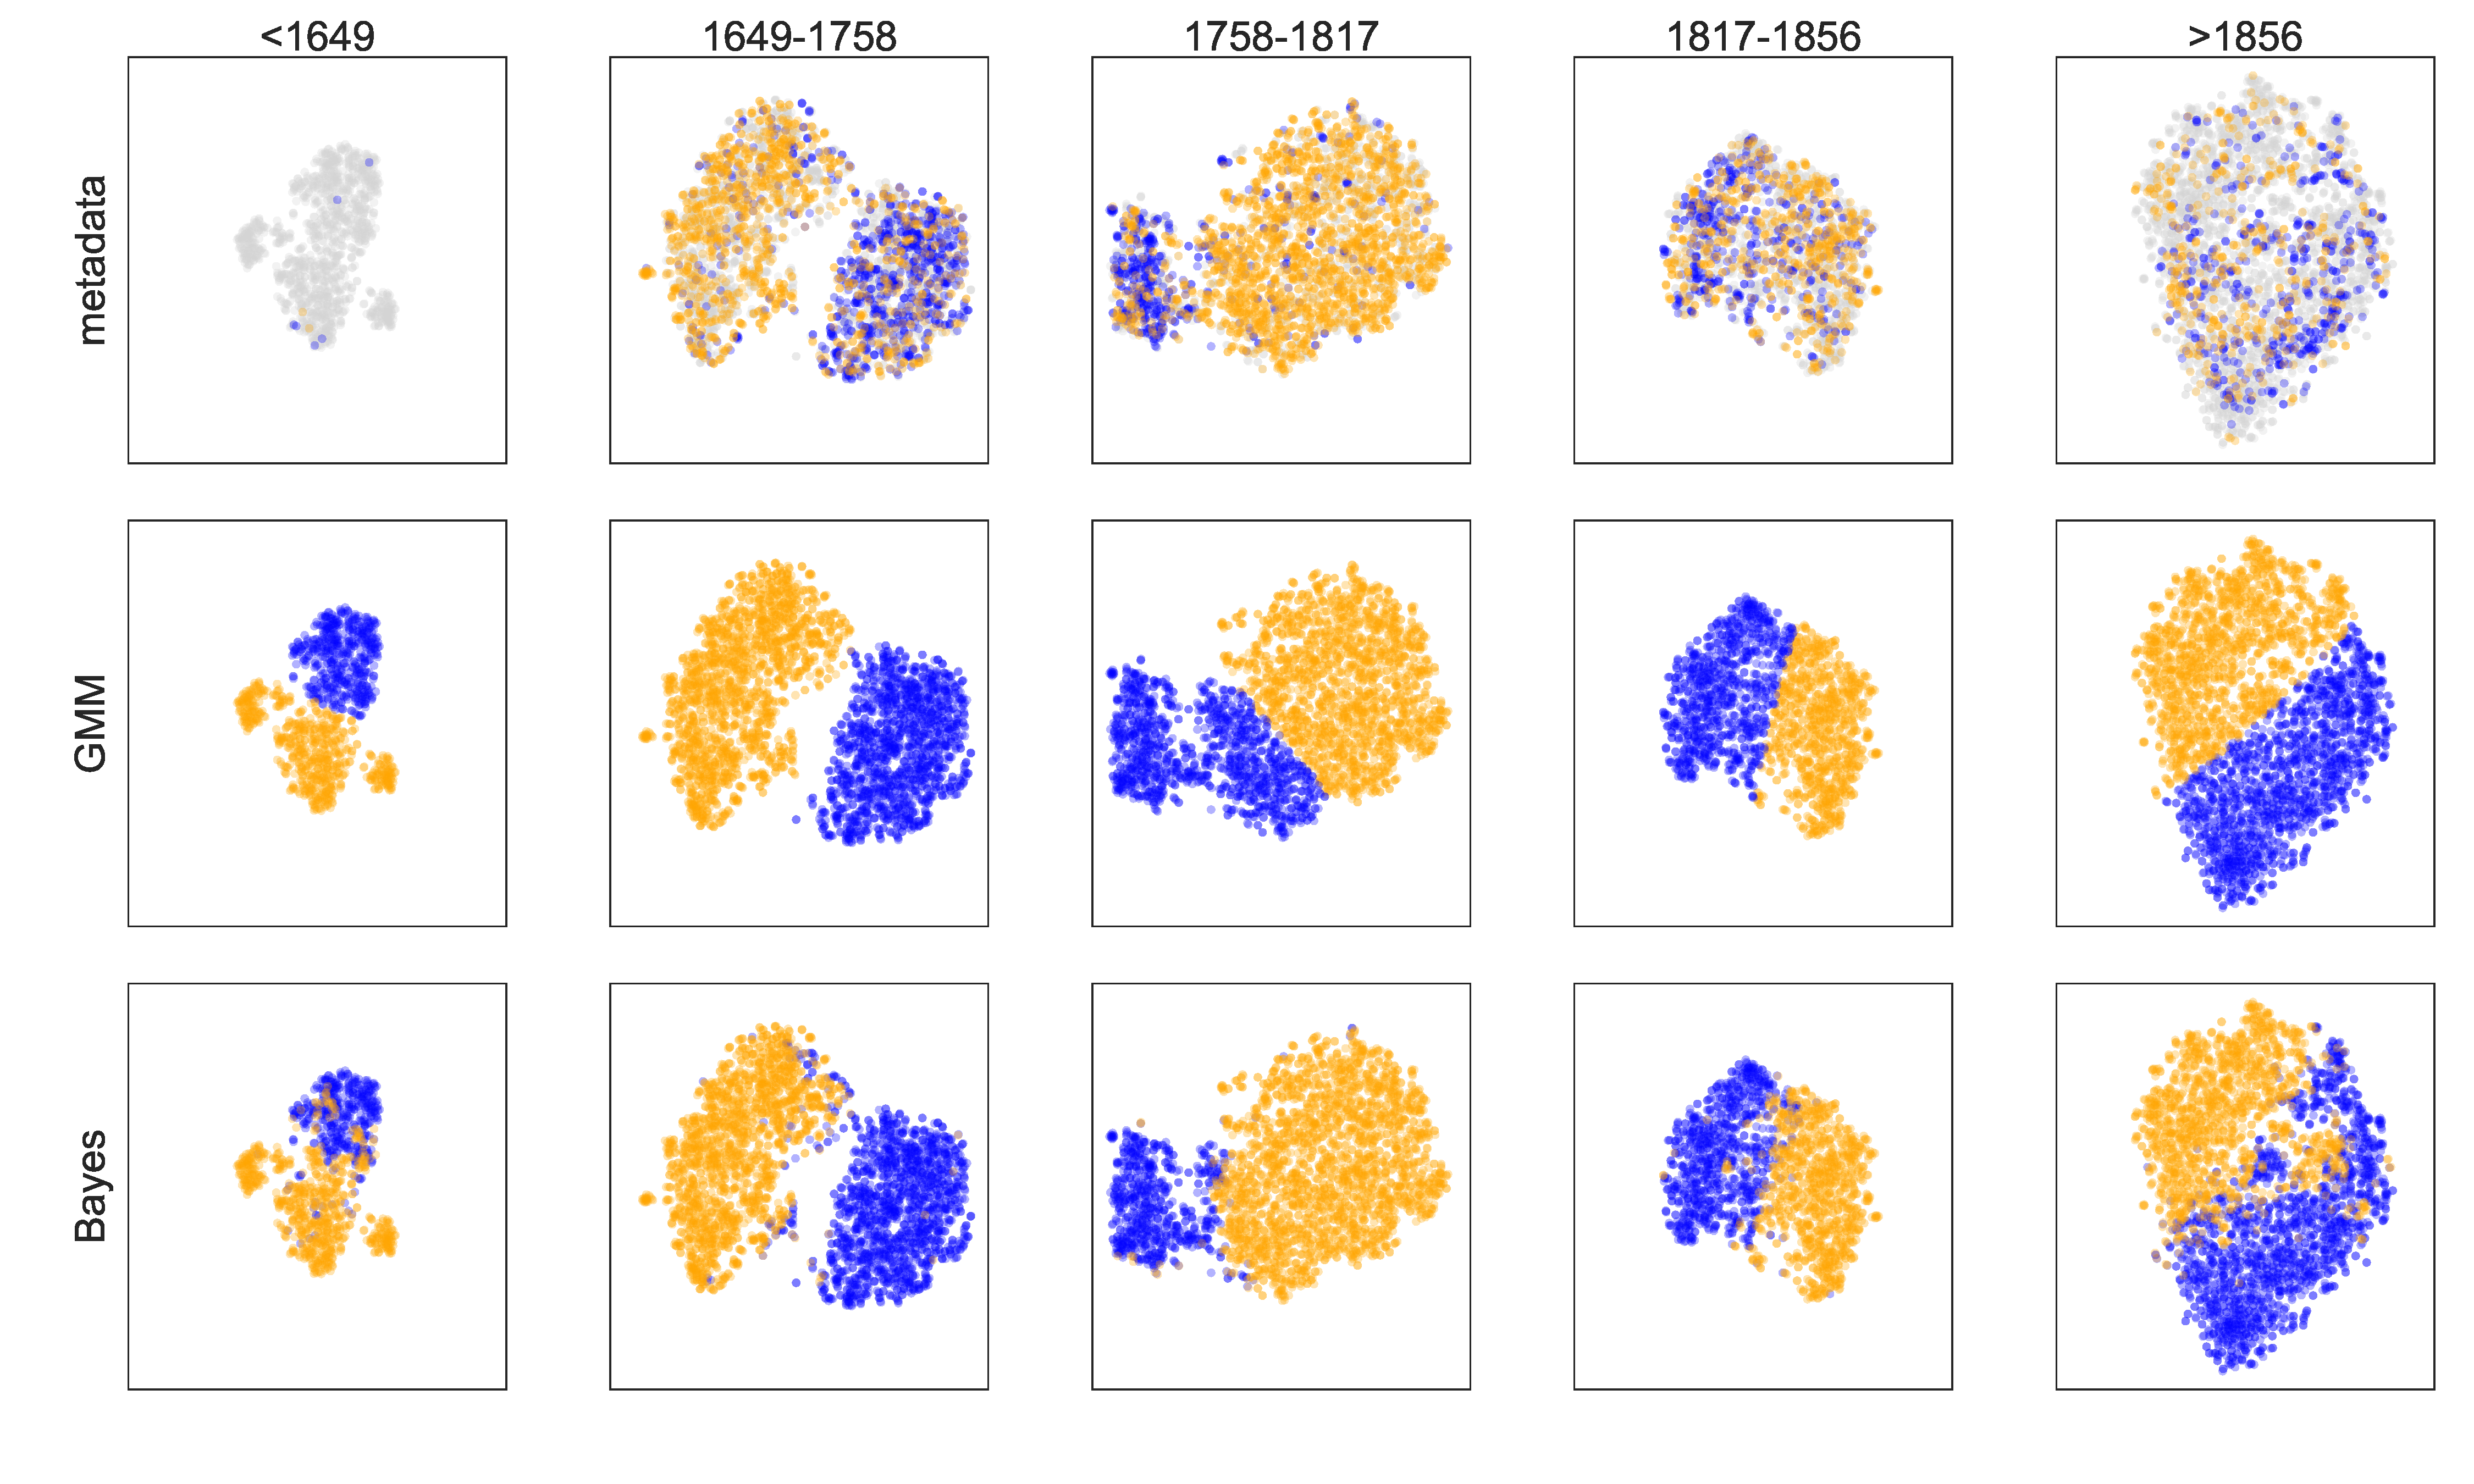
\includegraphics[width=\linewidth,height=.8\textheight,keepaspectratio]{img/Figure4.pdf}
        \caption{Three models for automatic mode finding.}
        % \label{fig:piece_dist}
    \end{figure}
\end{frame}

\begin{frame}{Quality of the model}
    \begin{figure}
        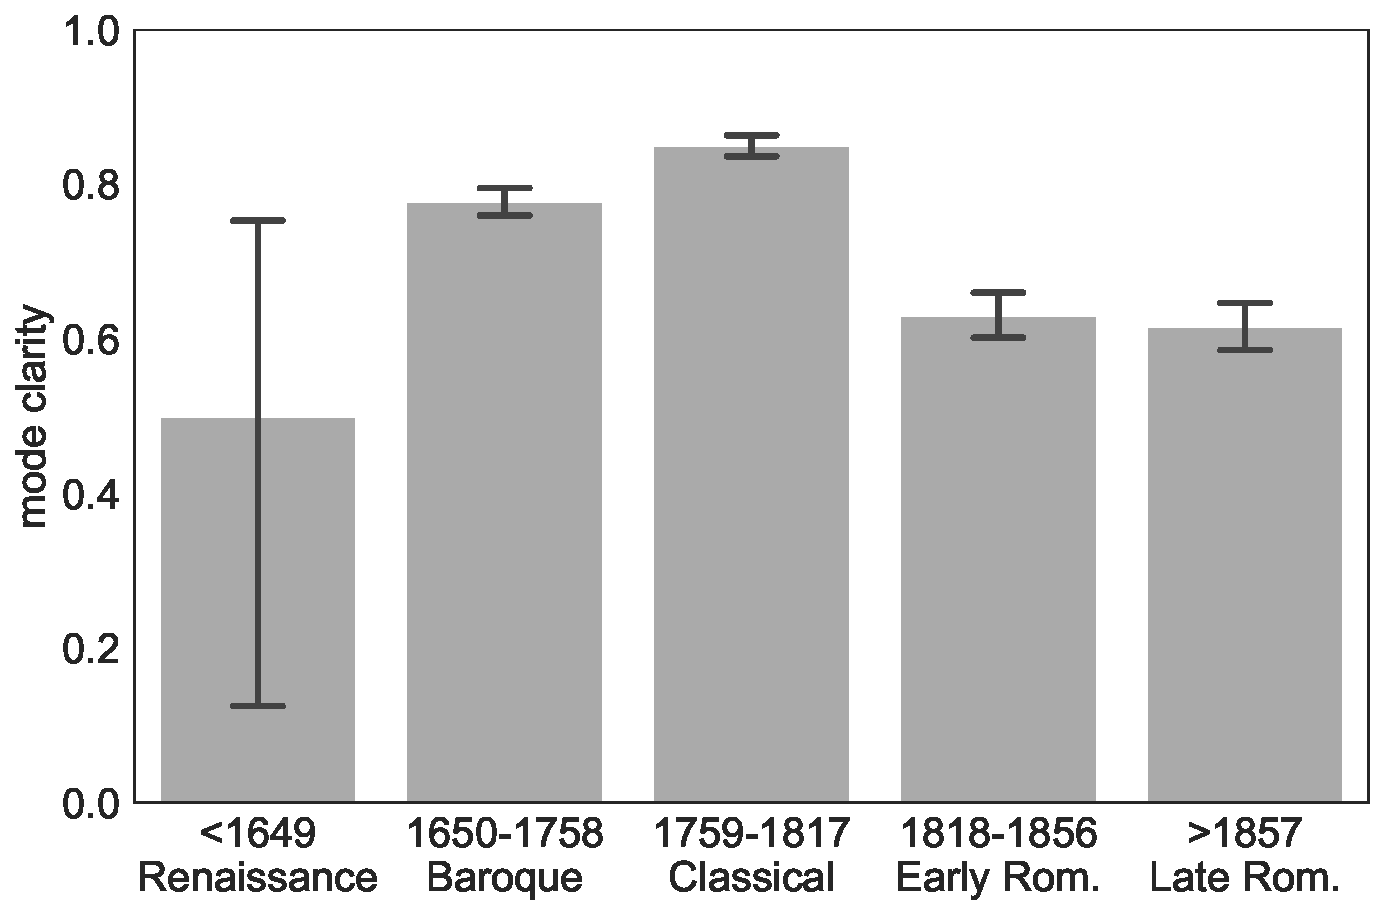
\includegraphics[width=\linewidth,height=.8\textheight,keepaspectratio]{img/Figure5.pdf}
        \caption{Accuracy scores of our model in five historical periods.}
        % \label{fig:piece_dist}
    \end{figure}
\end{frame}

\begin{frame}{The major and minor modes}
    \begin{figure}
        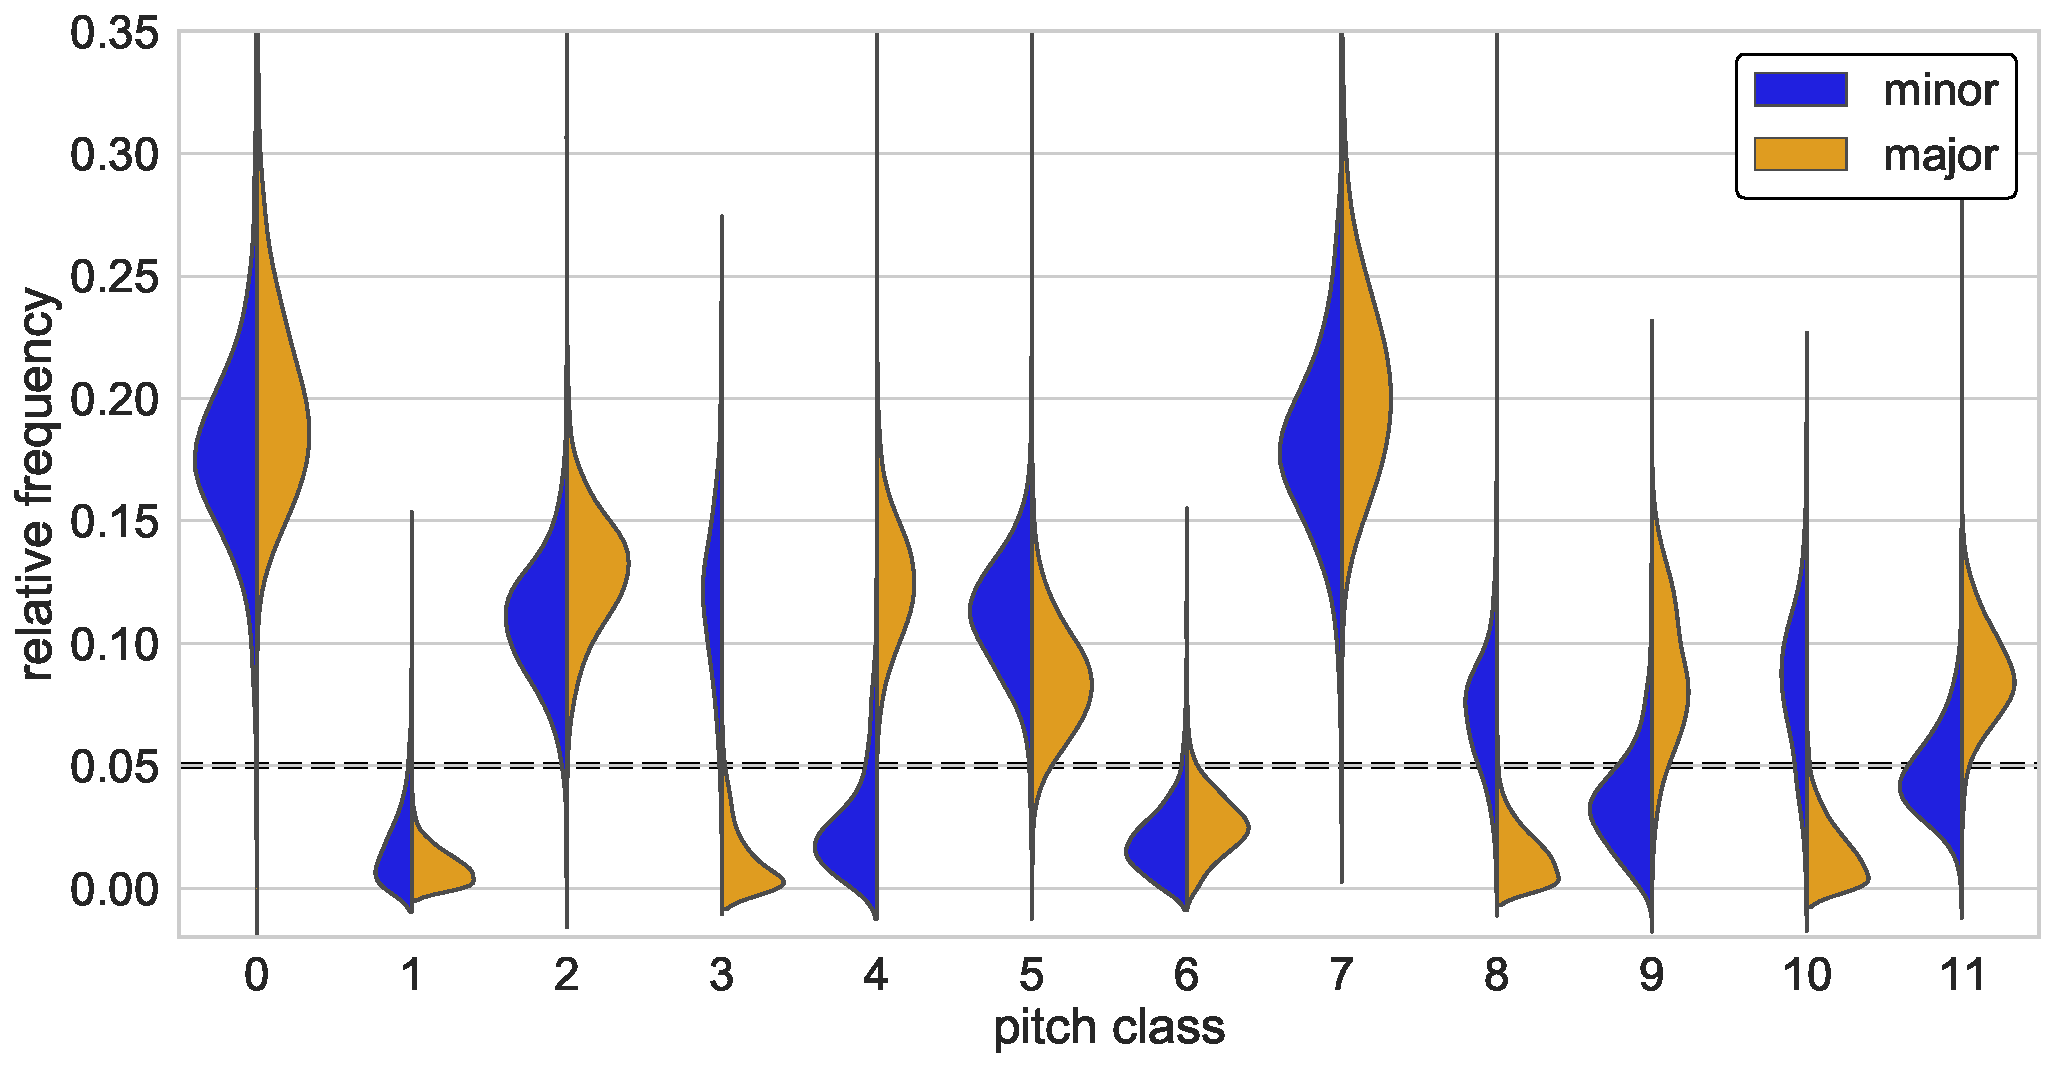
\includegraphics[width=\linewidth,height=.8\textheight,keepaspectratio]{img/Figure8.pdf}
        \caption{Pitch-class distribution of the major and minor modes.}
        % \label{fig:piece_dist}
    \end{figure}
\end{frame}

\begin{frame}{Modes in the Renaissance}
    \begin{figure}
        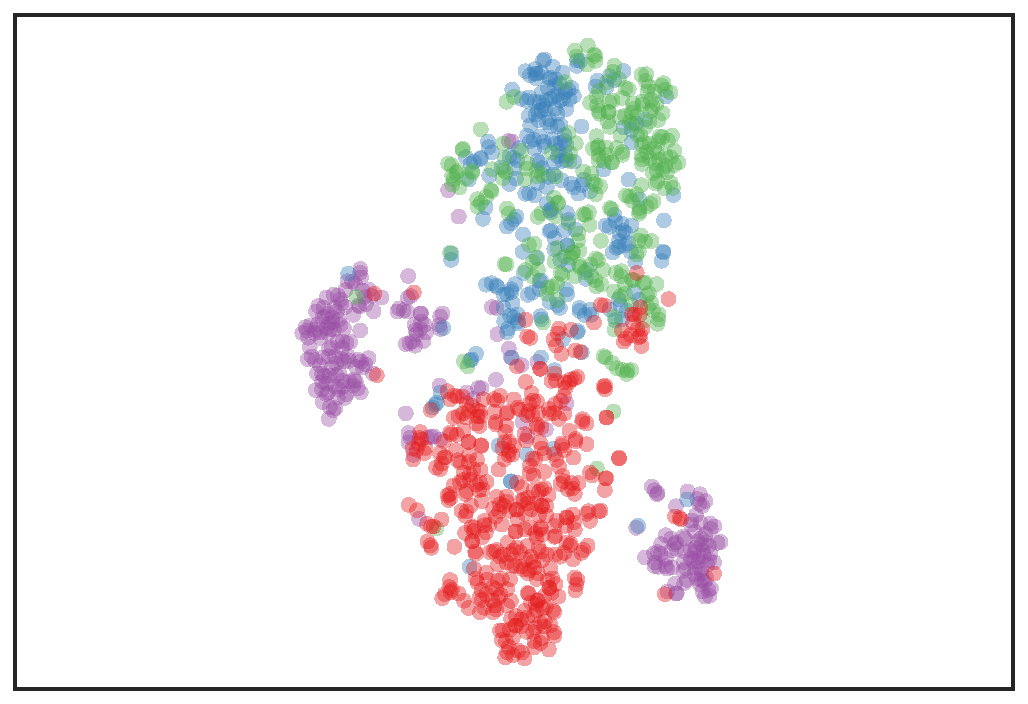
\includegraphics[width=\linewidth,height=.8\textheight,keepaspectratio]{img/Figure6.pdf}
        \caption{Clustering into four modes in the Renaissance.}
        % \label{fig:piece_dist}
    \end{figure}
\end{frame}

\begin{frame}{Modes in the Renaissance}
    \begin{figure}
        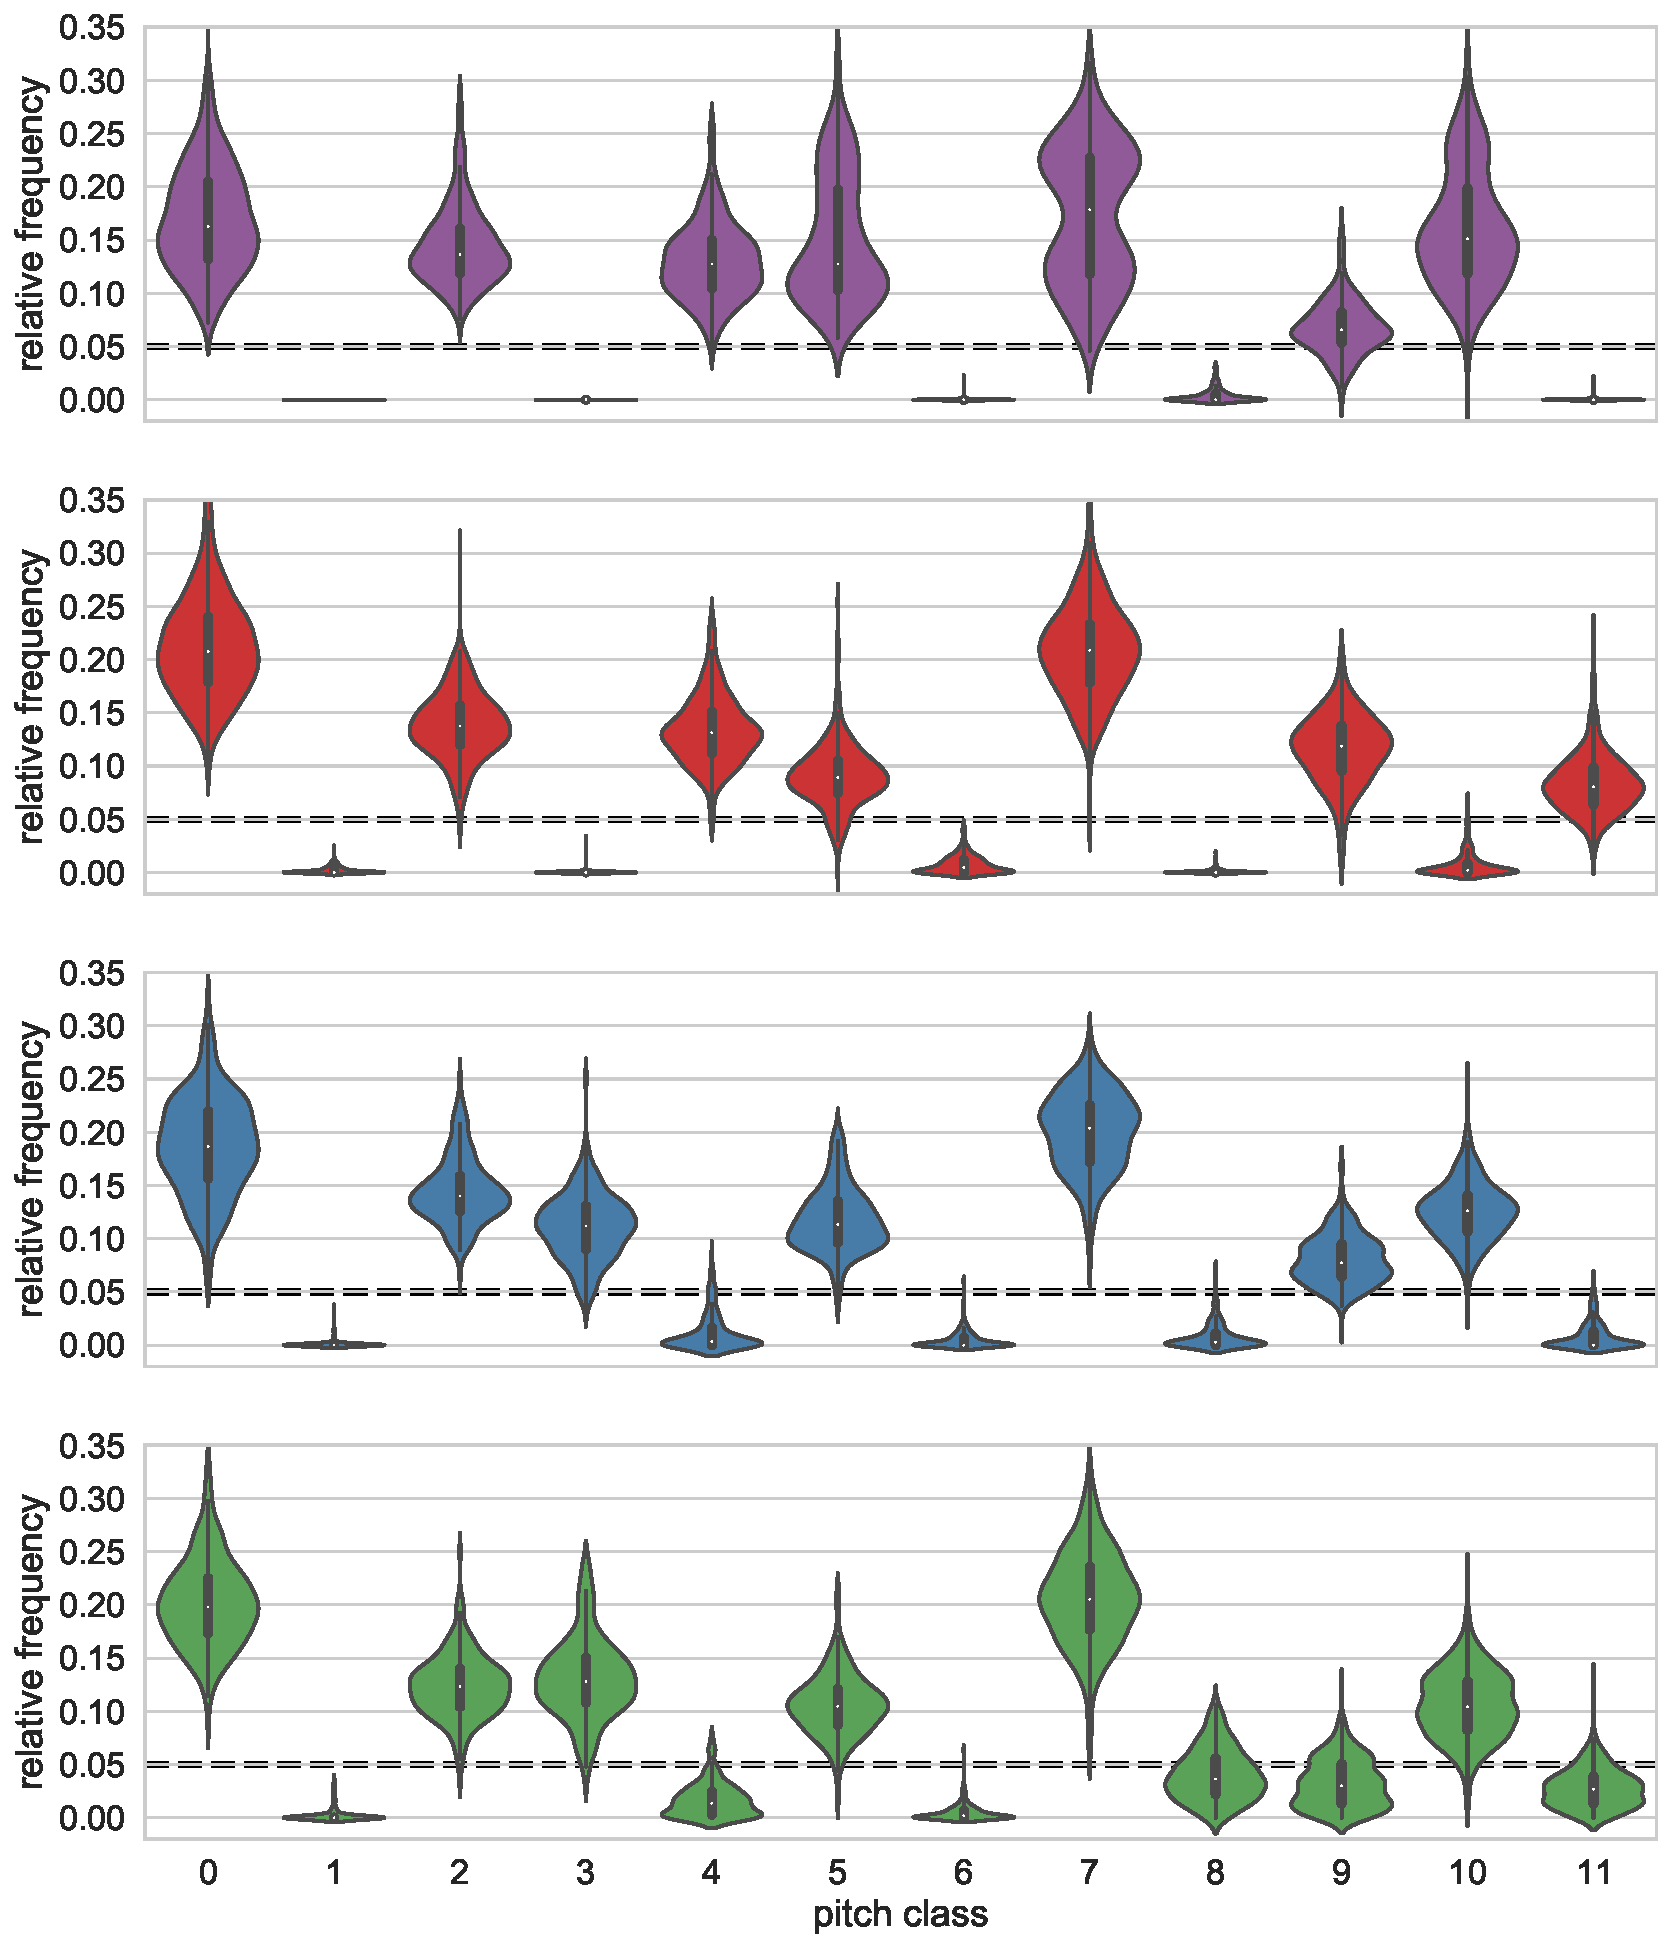
\includegraphics[width=\linewidth,height=.8\textheight,keepaspectratio]{img/Figure7.pdf}
        \caption{Pitch-class distribution of Renaissance modes.}
        % \label{fig:piece_dist}
    \end{figure}
\end{frame}